% don't remove the folling lines, and edit the defintion of \main if needed
\documentclass[../report.tex]{subfiles}
\providecommand{\main}{..}
\IfEq{\jobname}{\currfilebase}{\AtEndDocument{\biblio}}{}
% until here

\begin{document}

\section{Conclusions and Outlook}
\subsection{Higgs properties and EW phenomena at the HL-LHC}
The determination of Higgs boson properties, and their connection to electroweak symmetry breaking (EWSB), is a primary target of the HL-LHC physics programme. Since 2012, the Higgs physics programme has rapidly expanded, with new ideas, more precise predictions and improved analyses, into a major program of precision measurements, as well as searches for rare production and decay processes. Outstanding opportunities have emerged for measurements of fundamental importance, such as the first direct constraints on the Higgs trilinear self-coupling and the natural width. The HL-LHC programme covers also searches for additional Higgs bosons in EWSB scenarios motivated by theories beyond the SM (BSM). Finally, a rigorous effective field theory (EFT) framework allows one to parametrise in a model independent way all EW and Higgs results. 
The studies presented in this report update the key expectations for HL-LHC,  and summarise the interpretation of the future constraints on new physics in terms of EFT couplings. This reappraisal of the future sensitivities relies on the Run~2 analyses improvements and assumes the detector performance targets established in the experiments' upgrade TDRs.
%that the experiments' upgrades will compensate the performance loss due to the pile-up, which was the design goal of the upgrades. 
Further improvements should be possible with analyses optimised for the HL-LHC data sets.

The main Higgs boson measurement channels correspond to five production modes (the gluon fusion ggF, the vector boson fusion VBF, the associated production with a vector boson $WH$ and $ZH$, and the associated production with a pair of top quarks $ttH$) and seven decay modes: $H \to \gamma\gamma$, $ZZ^*$, $WW^*$, $\tau^+\tau^-$, $b\overline{b}$, $\mu^+\mu^-$ and $Z\gamma$. The latter two decay channels, as yet unobserved, should become visible during the next two LHC runs. 
The rate measurements in the aforementioned production and decay channels yield measurements of the Higgs couplings in the so-called "$\kappa$-framework". This introduces a set of $\kappa_i$ factors that linearly modify the coupling of the Higgs boson to SM elementary particles, $i$, including the effective couplings to gluons and photons, and assuming no additional BSM contribution to the Higgs total width, $\Gamma_H$. The projected uncertainties, combining ATLAS and CMS, are summarised in Fig.~\ref{fig:summary_K2} of Section~\ref{sec2}. They include today's theory uncertainties reduced by a factor of two, which is close to the uncertainty that would result from using the improved HL-LHC parton distribution functions (PDFs, see Section~\ref{sec2:PDFuncertainties}) and considering signal theory uncertainties as uncorrelated. Except for rare decays, the overall uncertainties will be dominated by the theoretical systematics, with a precision close to percent level.

The main Higgs boson couplings will be measured at HL-LHC with a precision at the percent level. Large statistics will particularly help the study of complex final states, such as those arising from $ttH$ production. 
The constraining power of the current $ttH$ analyses has been limited to plausible improvements in the theory predictions, in particular in the $H\rightarrow b\overline{b}$ channel. The 3.4\% precision on $\kappa_t$ thus obtained is mostly due to the other direct $ttH$ measurement channels.

%\begin{figure}
%\begin{center}
%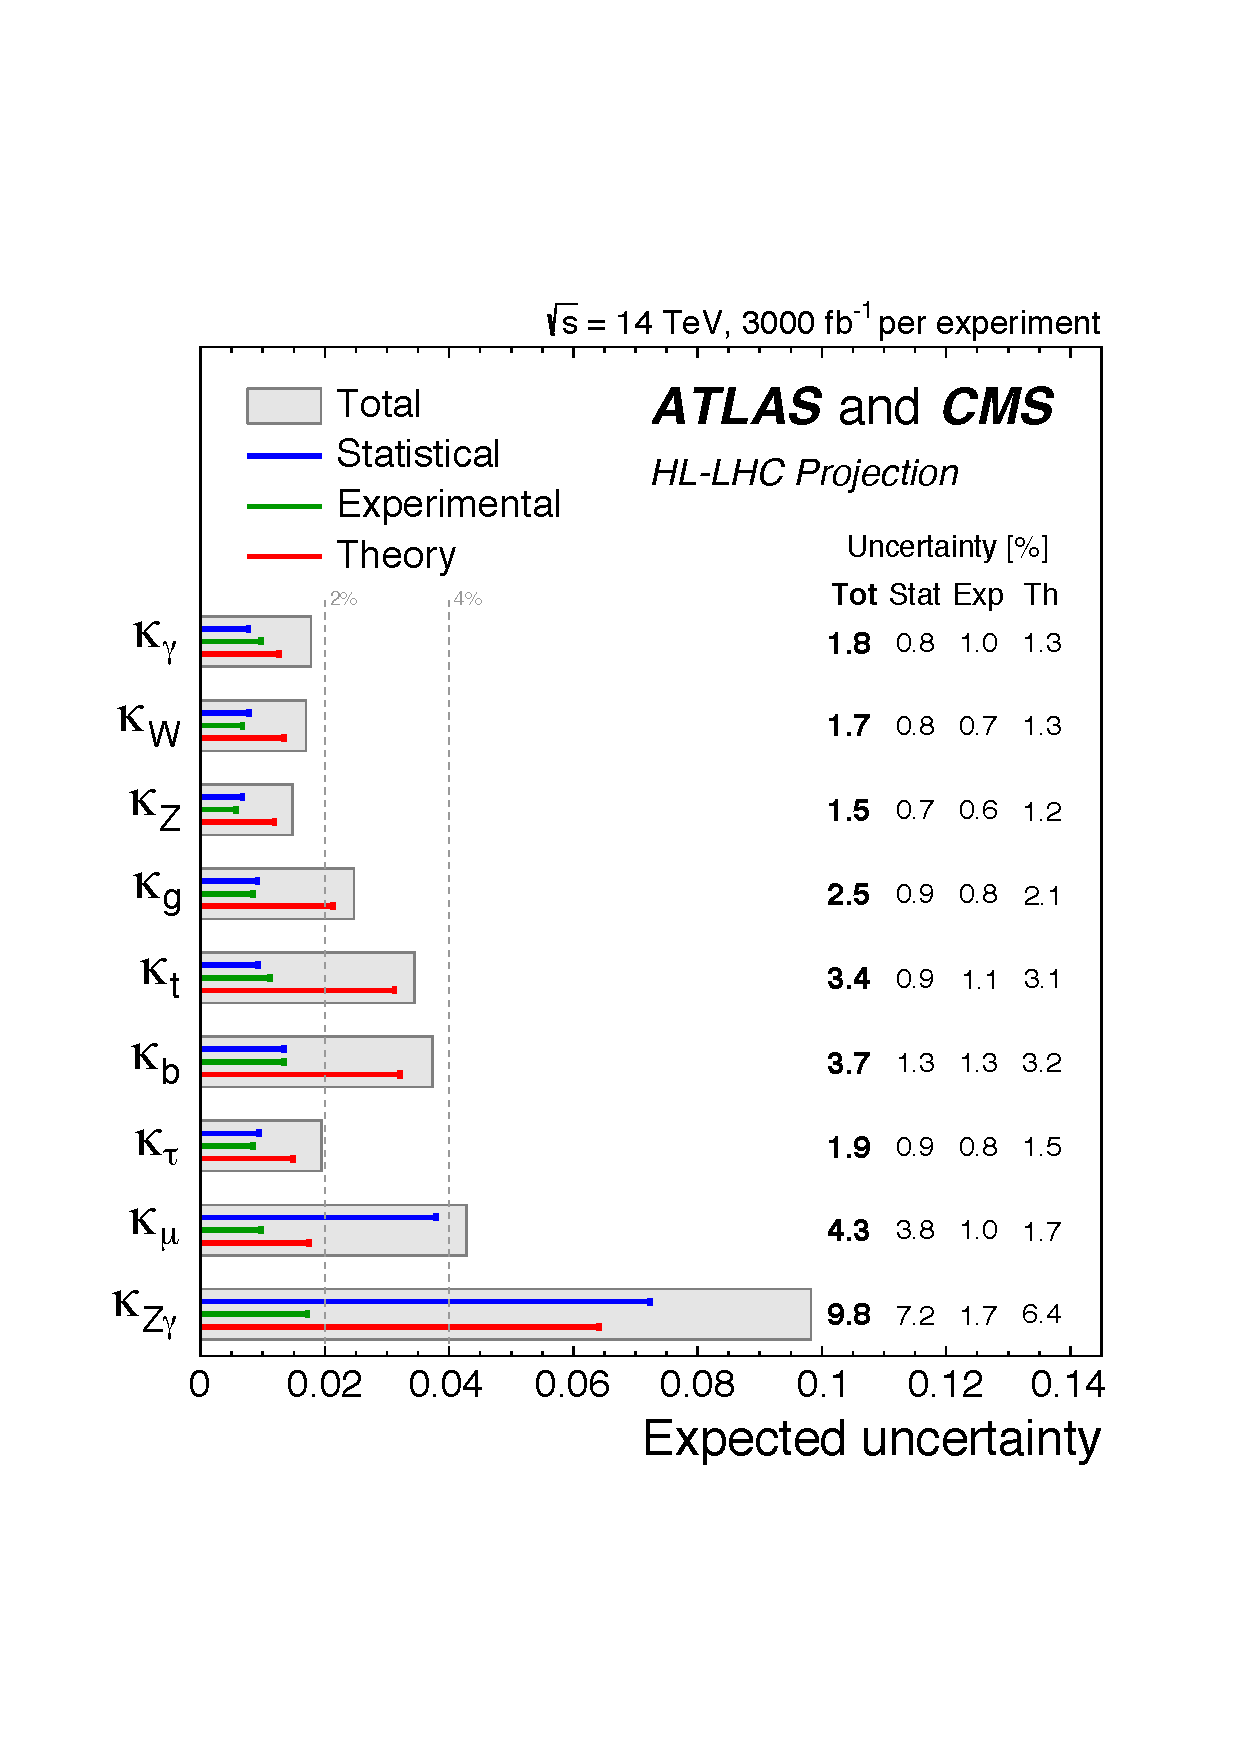
\includegraphics[width=0.60\textwidth,trim=1.3cm 3.3cm 1.3cm %5cm,clip]{section10/img/Kappas}
%\caption{Projected  uncertainties on $\kappa_i$, combining ATLAS and CMS: %total (grey box), statistical (blue), experimental (green) and theory (red). %See Section~\ref{sec2} for details.
%\label{fig:HiggsCouplings}
%}
%\end{center}
%\vskip -4mm
%\end{figure}

These coupling measurements assume the absence of sizeable additional contributions to $\Gamma_H$. As recently suggested, the patterns of quantum interference between background and Higgs-mediated production of photon pairs or four leptons are sensitive to $\Gamma_H$. Measuring the off-shell four-fermion final states, and assuming the Higgs couplings to gluons and $ZZ$ evolve off-shell as in the SM, the HL-LHC will extract $\Gamma_H$ with a 20\% precision at 68\%~CL.
Furthermore, combining all Higgs channels, and with the assumption that the couplings to vector bosons are not  larger than the SM ones ($\kappa_V\le 1$), will constrain $\Gamma_H$ with a 5\% precision at 95\%~CL. Invisible Higgs boson decays will be searched for at HL-LHC in all production channels, VBF being the most sensitive. The combination of ATLAS and CMS Higgs boson coupling measurements will set an upper limit on the Higgs invisible branching ratio of 2.5\%, at the 95\% CL.  The precision reach in the measurements of ratios will be at the percent level, with particularly interesting measurements of $\kappa_{\gamma}/\kappa_{\rm Z}$, which serves as a probe of new physics entering the $H \rightarrow \gamma\gamma$ loop, can be measured with an uncertainty of 1.4\%, and $\kappa_{t}/\kappa_{g}$, which serves as probe of new physics entering the $gg \rightarrow H$ loop, with a precision of 3.4\%.

%Measuring the first and second generation Yukawas is an important step in testing the fundamental nature of the observed Higgs-like boson. 
A summary of the limits obtained on  first and second generation quarks from a variety of observables is given in Fig.~\ref{fig:sec7:summary} of section~\ref{sec7}. It includes: (i) HL-LHC projections for {\it exclusive} decays of the Higgs into quarkonia; (ii) constraints from fits to differential cross sections of {\it kinematic} observables (in particular $p_\mathrm{T}$); (iii) constraints on the total {\it width}, $\Gamma_H$, relying on different assumptions (the examples given in  Fig.~\ref{fig:sec7:summary} correspond to a projected limit of 200~\UMeV on the total width from the mass shift from the interference in the di-photon channel between signal and continuous background and the constraint at 68\% CL on the total width from off-shell couplings measurements of 20\%); (iv) a {\it global} fit of Higgs production cross sections (yielding the constraint of 5\% on the width mentioned herein); and (v) the {\it direct search} for Higgs decays to $c\overline{c}$ using inclusive charm tagging techniques. Assuming SM couplings, the latter is expected to lead to the most stringent upper limit of $\kappa_c \lessapprox 2$. A combination of ATLAS, CMS and LHCb results would further improve this constraint to $\kappa_c \lessapprox 1$.
% PHIL version: Assuming SM couplings, these observables are expected to lead only to upper limits, the most stringent being $\kappa_c \lessapprox 2$, from a global fit and direct searches using $c$-tagged jets. A combination of ATLAS, CMS and LHCb direct search results could bring this to the SM level.

%\begin{figure}[b!]
%\begin{center}
%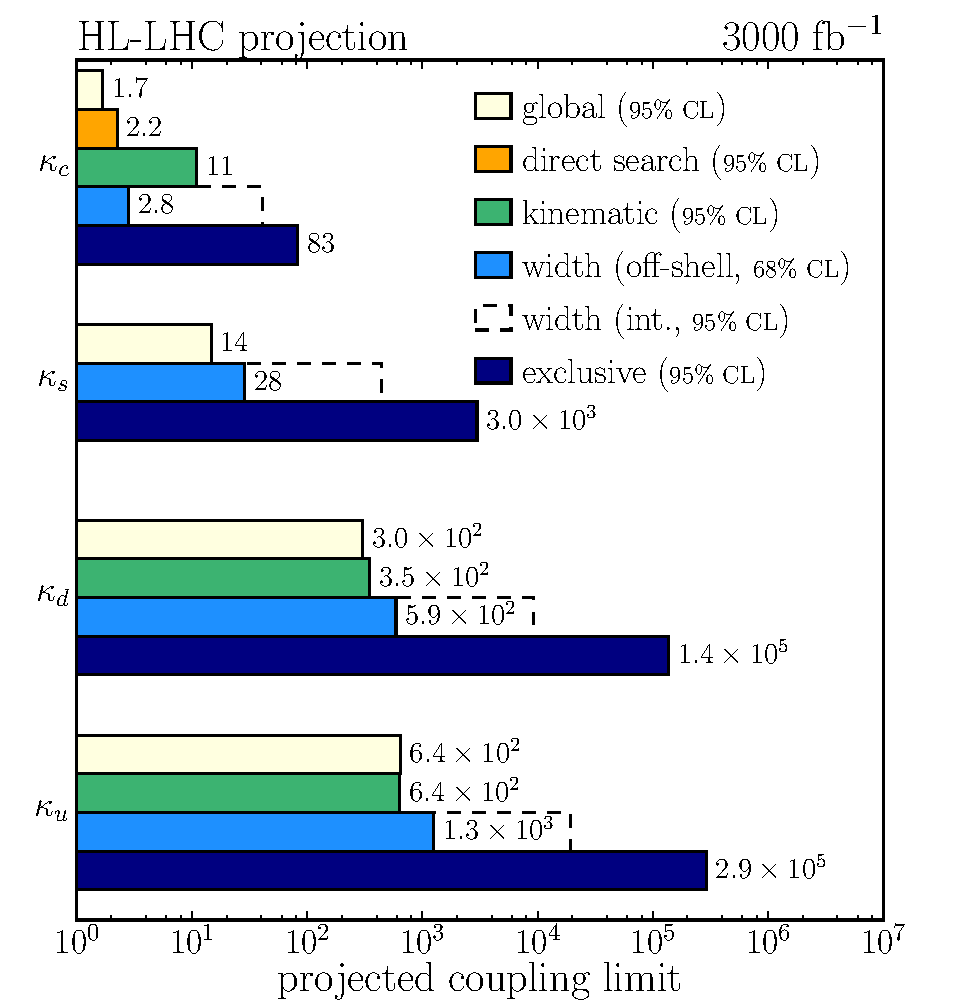
\includegraphics[width=0.50\textwidth]{section10/img/Yukawa} 
    %\caption{Summary of the projected HL-LHC limits on the quark
     % Yukawa couplings. See Section~\ref{sec7} for details. %\label{fig:HiggsFlavor}
 %     }
%\end{center}
%\end{figure}

%\begin{figure}
%\begin{center}
%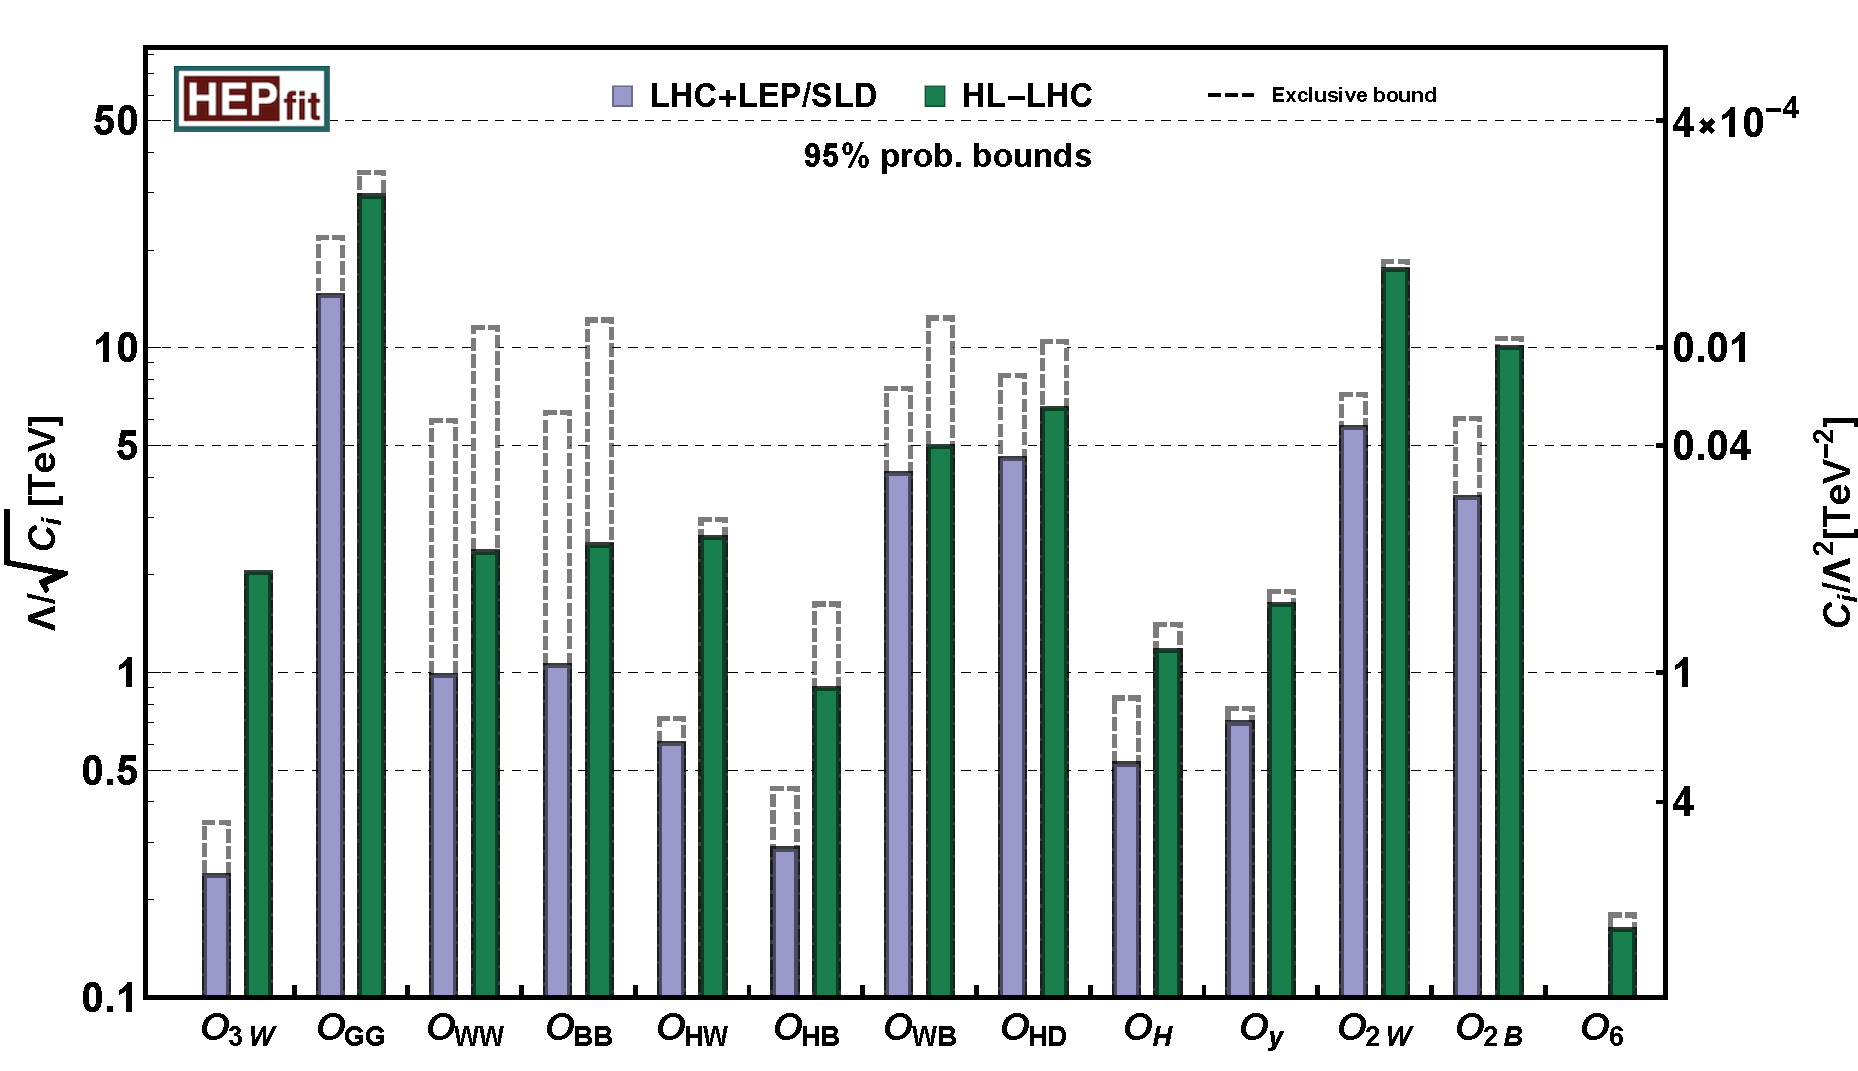
\includegraphics[width=0.85\textwidth,trim=0cm 0cm 0cm %0.7cm,clip]{section10/img/EFT.pdf}
%    \includegraphics[width=0.65\textwidth]{mass}
%\vspace{2mm}
    %\caption{Summary of constraints on the SMEFT operators   considered. The %shaded bounds arise from a global fit of all operators, those assuming %the existence of a single operator are labeled as "exclusive". See %Section~\ref{sec8:globalfit} for details.\label{fig:HiggsEFT}
 %   }
%\end{center}    
%\end{figure}
%{fig:dim6U_HLLHC}

Precision measurements provide an important tool to search for BSM physics associated to mass scales beyond the LHC direct reach. The EFT framework, where the SM Lagrangian is supplemented with dimension-6 operators $\sum_{i} c_i \mathcal{O}^{(6)}_i/\Lambda^2$, allows one to systematically parametrise BSM effects and how they modify SM processes. Figure~\ref{fig:dim6U_HLLHC} of section~\ref{sec8:globalfit} shows the results of a global fit  to observables in Higgs physics, as well as di-boson and Drell-Yan processes at high energy. The fit includes all operators generated by new physics that only couples to SM bosons. These operators can either modify SM amplitudes, or generate new amplitudes. In the former case, the best LHC probes are, for example, precision measurements of Higgs branching ratios. In the case of the operator $\mathcal{O}_H$, 
for example, the constraints in Fig.~\ref{fig:dim6U_HLLHC} translate into a sensitivity to the Higgs compositeness scale $f>1.6$~\UTeV, corresponding to a new physics mass scale of 20~\UTeV for an underlying strongly coupled theory.
The effects associated with some new amplitudes grow quadratically with the energy. For example, Drell-Yan production at large mass can access, via the operators $\mathcal{O}_{2W,2B}$, energy scales of order 12~\UTeV (Fig.~\ref{fig:dim6U_HLLHC}). 

The Run~2 experience in searches for Higgs pair production led to a reappraisal of the HL-LHC sensitivity, including several channels, some of which were not considered in previous projections: $2\textrm{b}2\gamma$, $2\textrm{b}2\tau$, $4\textrm{b}$, $2\textrm{b}\textrm{WW}$, $2\textrm{b}\textrm{ZZ}$.
Assuming the SM Higgs self-coupling $\lambda$, ATLAS and CMS project a sensitivity to the $HH$ signal of approximately 3 $\sigma$. per experiment, leading to a combined observation sensitivity of 4 $\sigma$. These analyses, which make use also of the $HH$ mass spectrum shape, result in the likelihood profile as a function of $\kappa_{\lambda}$ shown in Fig.~\ref{fig:comb_HH} of section~\ref{sec:HH_Combination}. An important feature of these analyses is the presence of the secondary minimum in the likelihood line-shape, due to the degeneracy in the total number of $HH$ signal events for different $\kappa_{\lambda}$ values. We note that at the HL-LHC the secondary minimum can be excluded at 99.4\%~CL, with a constraint on the Higgs self-coupling of $0.5 < \kappa_{\lambda} < 1.5 $ at the 68\%\ CL. The results on HH production studies are statistics limited, therefore a dataset of at least 6\,\iab{}  (ATLAS and CMS combined) is essential to achieve this objective.

%\begin{figure}[t!]
%\begin{center}
% 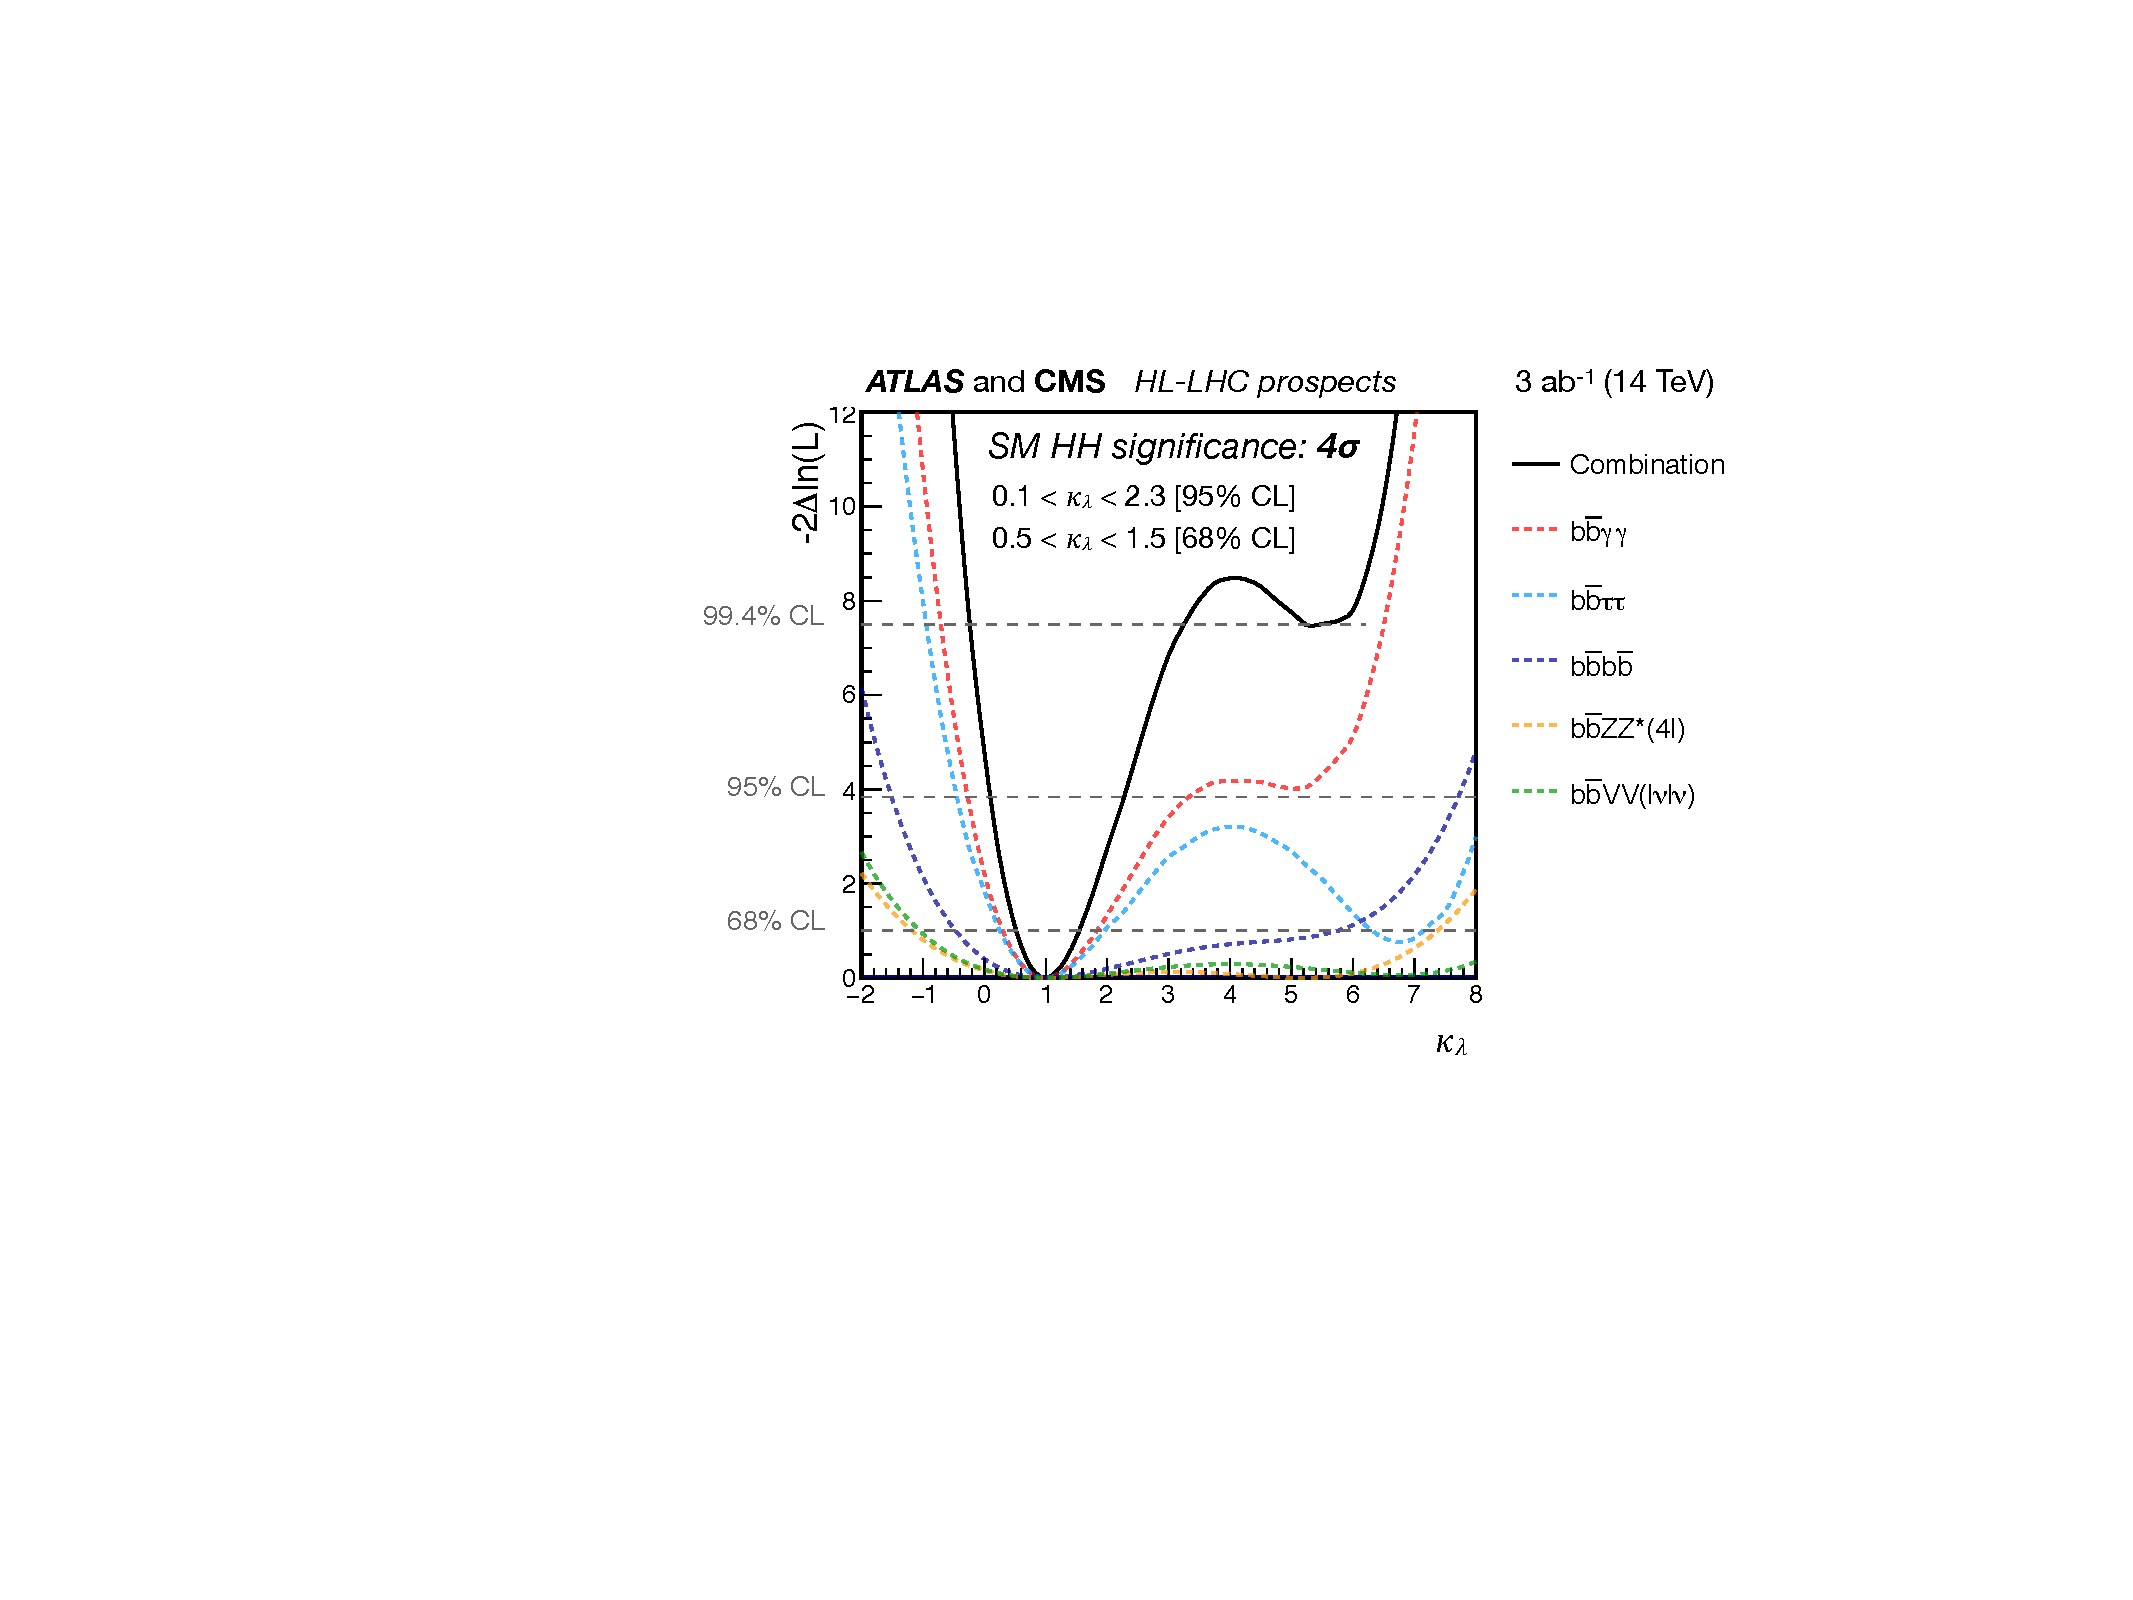
\includegraphics[width=0.85\textwidth]{section10/img/HH.pdf}
% \caption{Projected combined HL-LHC sensitivity to Higgs trilinear coupling %from direct search channels. See Section~\ref{sec:HH_Combination} for %details.
%\label{fig:HiggsHH}
%}
%  \end{center}
%\end{figure}
%{fig:comb_HH}


%\begin{figure}[t!]
%\begin{center} 
%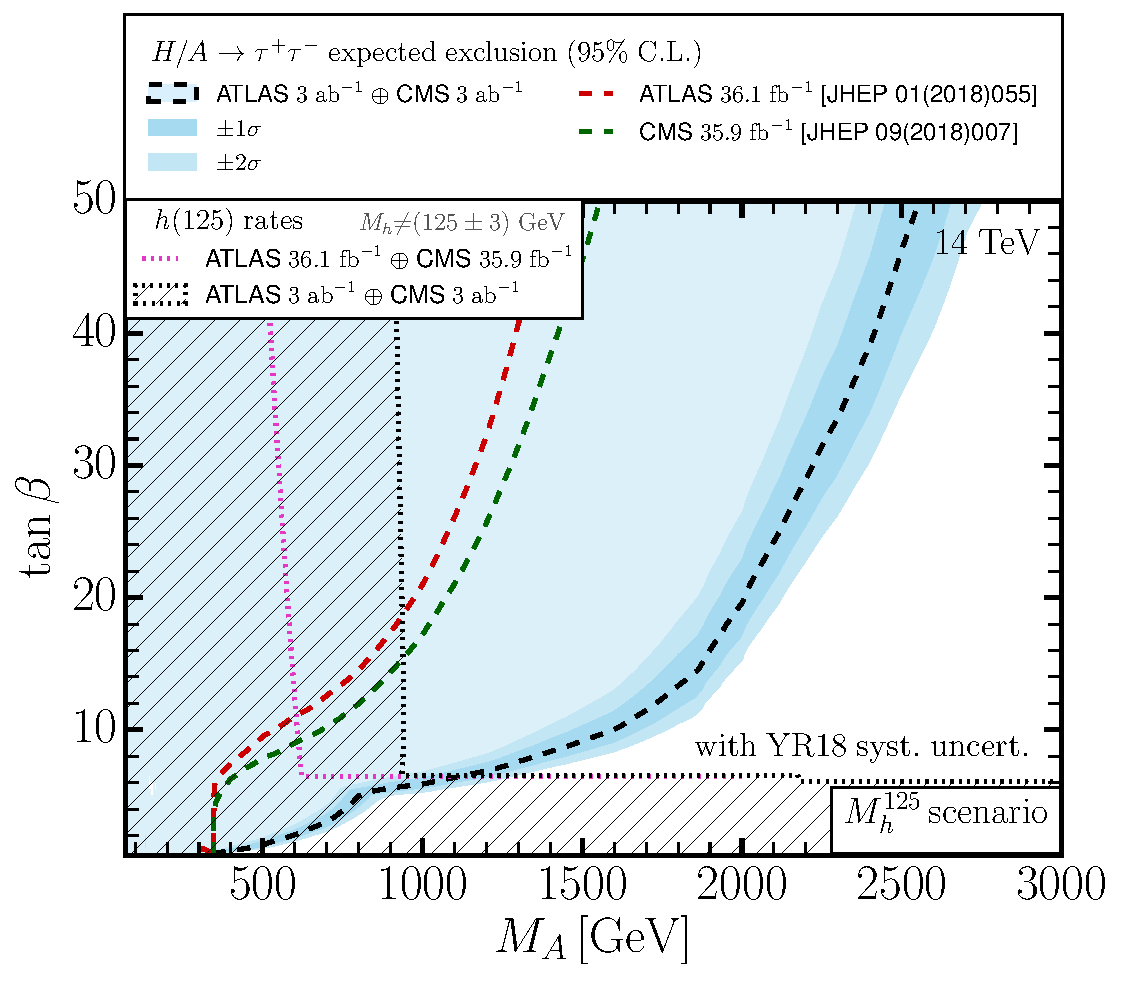
\includegraphics[width=0.85\textwidth]{section10/img/BSM.pdf}
%\caption{Sensitivity to BSM Higgs bosons, in the $H/A\to\tau\tau$ channel. %See Section~\ref{sec9} for details.
%\label{fig:HiggsBSM}
% }
%  \end{center}
%\end{figure}
%Fig.~\ref{fig:bench}

Higgs studies at HL-LHC will enhance the sensitivity to BSM physics, exploiting indirect probes via precision measurements, and a multitude of direct search targets, ranging from exotic decays of the 125~\UGeV Higgs boson (e.g. decays including promptly decaying light scalars, light dark photons or axion-like particles, and decays involving long-lived BSM particles) to the production of new Higgs bosons, neutral and charged, at masses above or below 125~\UGeV.
%BSM theories generically predict the Higgs couplings to deviate from the SM predictions. The HL-LHC precision will lead to stringent constraints, e.g. on the scale of compositeness in composite Higgs models. In parallel, the HL-LHC will have a very broad reach on models predicting rare 125 GeV Higgs boson exotic decays (examples are decays including intermediate BSM particles that are long lived, decays including light scalars, light dark photons or axion-like particles).
%Extended Higgs sectors can be tested either indirectly through precision Higgs measurements or directly through searches.  These machines will cover much larger regions of parameter space of models with new heavy ($m_H>125$ GeV) neutral of charged Higgs bosons, as well as new light ($m_H < 125$ GeV) Higgs bosons. Examples are the searches for SUSY heavy Higgs bosons decaying into a $\tau\tau$ pair at ATLAS and CMS and the searches for light Higgs bosons decaying into a $\mu\mu$ pair at LHCb.
The HL-LHC will be able to probe very rare exotic decay modes of the 125 \UGeV Higgs boson thanks to the huge Higgs data set that will be produced (branching ratios as small as $\mathcal O(10^{-6})$ could be probed for sufficiently clean decay modes). Furthermore, the mass reach for new heavy Higgs bosons can be pushed to few \UTeV. As an example, Fig.~\ref{fig:bench} in section~\ref{Sec:9.5}, shows a summary of the Minimal Supersymmetric SM regions of parameter space that will be probed by ATLAS and CMS either via direct searches of new Higgs bosons decaying to tau lepton pairs, or via indirect 125 \UGeV Higgs coupling measurements. The HL-LHC will have access to new Higgs bosons as heavy as ~2.5 \UTeV at large $\tan\beta$ ($\tan\beta>50$). Complementarily, the interpretation of Higgs precision coupling measurements will exclude Higgs bosons with masses lower than approximately 1~\UTeV over a large range of $\tan\beta$.

\subsection{Potential of the HE-LHC}
With the increase in centre-of-mass energy and luminosity, the Higgs physics programme at HE-LHC will considerably extend the reach of the entire HL-LHC program. Measurements of the Higgs boson trilinear self-coupling, of elusive decay modes (e.g.\,H$\to$c\={c}), of rare (e.g.\,H$\to$Z\textgamma), invisible or exotic decays will become accessible. At the same time, Higgs boson production can be explored at very large transverse momenta.
%With the increase in centre-of-mass energy and luminosity, the Higgs physics programme at HE-LHC will considerably extend the precision reach of the entire HL-LHC program: with the measurement of the Higgs boson trilinear self-coupling, the measurement of elusive decay modes (e.g.\,H$\to$c\={c}), of rare (e.g.\,H$\to$Z\textgamma) and invisible or forbidden decays, and with the measurement of Higgs bosons produced at very large transverse momenta. 
Projections presented in this section are exploratory and provide qualitative results, due to the absence of clearly defined reference detectors, and in view of the highly challenging pile-up environment. Several approaches have been followed to address this issue, typically assuming experimental performances similar to those currently achieved by LHC detectors. Other studies focused on Higgs bosons produced at finite transverse momentum ($p_T>50$~\UGeV), to reduce the impact of pile-up. The selection of fiducial regions in $p_T$ and rapidity, furthermore, allows measurements of the ratios of rates for different final states, free of uncertainties related to the production dynamics and to luminosity. 

\begin{table}[h]
\centering
  \caption{\label{tab:Hrates}
Higgs production event rates for selected processes
    at 27~\UTeV ($N_{27}$) and
 statistical increase with 
 respect to the statistics of the HL-LHC ($N_{27}=\sigma_{27~\mathrm{\UTeV}} \times 15$~\iab, 
 $N_{14}=\sigma_{14~\mathrm{\UTeV}} \times 3$~\iab).} 
\begin{tabular}{|l|c|c|c|c|c|c|} 
\hline  \hline
&  gg\,$\to$\,H   & VBF &
 WH  &
 ZH  &
 $\rm t\bar{t}H$ &
 HH 
 \\ \hline
$N_{27}$  & $2.2\times 10^9$ & $1.8\times 10^8$ & $5.4\times 10^7$ & $3.7\times
 10^7$ &  $4\times 10^7$ & $2.1 \times 10^6$  \\
$N_{27}/N_{14}$ & 13 & 14 & 12 & 13 &23 & 19
\\ \hline
\hline
\end{tabular}
\end{table}
The statistics expected for some reference production processes, and the increase with respect to the HL-LHC, are shown in
Table~\ref{tab:Hrates}. The Higgs samples will typically increase by a factor between 10 and 25, in part as a result of the 5 times larger luminosity, leading to a potential reduction in the statistical uncertainties by factors of 3 to 5. The biggest improvements arise for the channels favoured by the higher energy, such as ttH and HH.

%\begin{figure}
%\begin{center}
%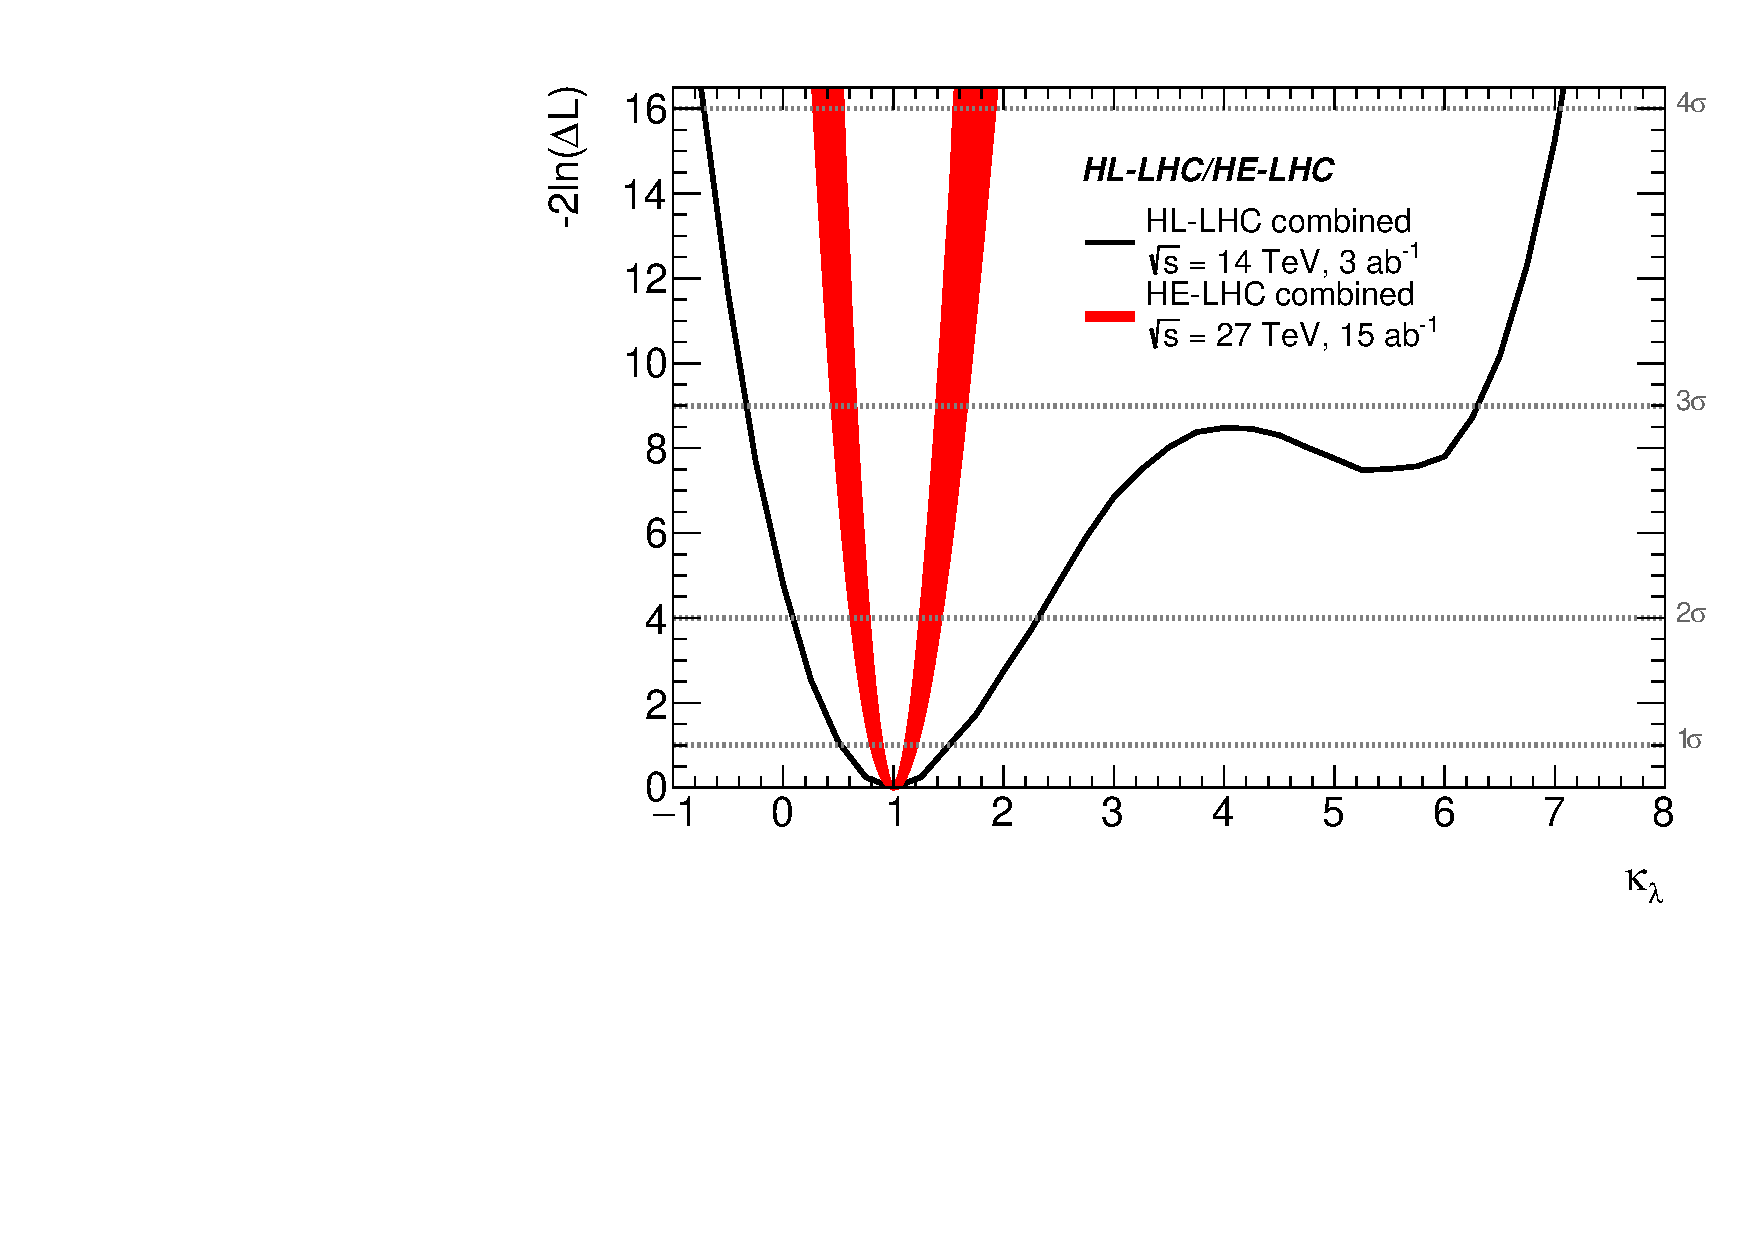
\includegraphics[width=0.65\textwidth]{section10/img/HH_HE-LHC.pdf}
%\caption{Expected sensitivity for the measurement of the of the Higgs %trilinear coupling through the measurement of direct $HH$ production at %HE-LHC. See Section~\ref{sec:HH_HE} for details.}
%\label{fig:HiggsHH_HE}
%\end{center}
%\end{figure}
%\ref{fig:HH_HELHC_comb}

The potential for the measurement of the Higgs boson trilinear coupling at the HE-LHC has been estimated with methods and in channels similar to those used at the HL-LHC. Extrapolation studies from the current experiments and from phenomenological studies have been carried out in the two most sensitive $HH$ channels at the HL-LHC ($b\overline{b}\gamma\gamma$ and $b\overline{b}\tau^+\tau^-$). 
Several studies were made under different experimental performance and systematic uncertainty assumptions (in some cases neglecting systematic uncertainties), yielding results covering the wide range of precision estimates presented here. At the HE-LHC the $HH$ signal would be observed unambiguously and the combined sensitivity on the trilinear coupling, $\kappa_{\lambda}$ (assuming the SM value), is expected to reach a precision of 10\% to 20\% from the combination of these two channels alone. A comparison of the HE-LHC sensitivity to that of the HL-LHC is displayed in Fig.~\ref{fig:HH_HELHC_comb} of section~\ref{sec:HH_HE}, showing that the secondary minimum still visible in the HL-LHC study is unambiguously excluded at HE-LHC. 
%It should be emphasized that these results rely on assumptions of experimental performance in very high pile up environment O(800-1000) that would require further validation with more detailed studies.
These studies do not include the additional decay channels that have already been studied for HL-LHC, and of others that could become relevant at the HE-LHC. Exclusive production modes are also very interesting to take into consideration for this measurement. The potential improvements from these have not been assessed yet.

The measurement of the couplings of the Higgs boson at HL-LHC relies either on the assumption that no additional undetected contribution to the Higgs boson width is present, or that the couplings of the Higgs boson to vector bosons do not exceed those expected in the SM. In both cases, the foreseen precision in the measurements of most Higgs boson couplings at the HL-LHC is currently limited by the theoretical uncertainty on the signal predictions. The significantly larger dataset and the increase in centre-of-mass energy at HE-LHC would reduce the statistical uncertainty of these measurements to being negligible.
%, offering unique opportunities for precision measurements provided that  significant improvements in the theoretical uncertainties on the signal predictions are achieved. The precision would otherwise not increase  with respect to HL-LHC 
To match the overall precision of the experimental measurements, the extraction of the couplings of the Higgs boson to photons, gluons, W, Z, taus, and b quarks will require significant theoretical improvements in the precision of the theoretical predictions for the signals.

%{\bf ***MLM: what are the quantities whose precision is reported in this paragraph? Is it the couplings, the kappa values, the BRs, ...?}
For rare decay processes such as the di-muon channel, from an extrapolation of the HL-LHC projections, a precision of approximately 2\% on the coupling modifier 
should be achievable.
 With the current theoretical systematic uncertainties on the signal and the backgrounds, the direct measurement of the Higgs coupling modifier to top quarks is expected to reach a precision of approximately 3\%. While the substantial additional amount of data at various centre-of-mass energies will undoubtedly be useful to further constrain the systematic modelling uncertainties and further progress in theoretical predictions will be achieved, the potential improvements have not been quantified. Assuming an improvement of the theoretical uncertainties of a factor of 2, the precision on the ttH coupling would reach approximately 2\% (the experimental systematic uncertainty alone is approximately 1\%, assuming performances similar to current LHC experiments). The significant gain in precision will be obtained mostly through ratios of couplings. Studies have shown that the ratio of the $t\overline{t}H$ to $t\overline{t}Z$ ratio could be measured at close to the percent level.

At HE-LHC energies, the $H \to c\bar{c}$ production increases relative to backgrounds, and may be observable with inclusive searches by ATLAS, CMS, and LHCb, depending on $c$-tagging systematic uncertainties. Unfortunately, at the HE-LHC, exclusive searches, kinematic limits, and global fits are not expected to reach the SM level for the $u$, $d$, $s$, and $c$ Yukawas.
%Unfortunately, exclusive searches, kinematic limits, and global fits are still not expected to reach the SM level for the $u$, $d$, $s$, and $c$ Yukawas.

Precision measurements provide an important tool to search for BSM physics associated to mass scales beyond the LHC direct reach. The EFT framework, where the SM Lagrangian is supplemented with higher dimension operators % $\sum_{i} c_i^{(6)}\mathcal{O}^{(6)}_i/\Lambda^2+c_i^{(8)}\mathcal{O}^{(8)}_i/\Lambda^4+\cdots$, 
allows one to systematically parametrise BSM effects and how they modify SM processes. These operators can either modify SM amplitudes, or generate new amplitudes. In the former case, the best LHC probes are, for example, precision measurements of Higgs branching ratios. In the case of the operator $\mathcal{O}_H$, for example, the constraints in Fig.~\ref{fig:dim6U_HELHC} of Section~\ref{sec8:globalfit}, translate into a sensitivity to the Higgs compositeness scale $f>2$~\UTeV, corresponding to a new physics mass scale of 25~\UTeV for an underlying strongly coupled theory.

Effects associated with  new amplitudes grow quadratically (for dimension-6 operators) with the energy. The higher centre-of-mass energy and larger dataset of HE-LHC make it possible to greatly extend the measurable range in the Higgs transverse momenta, providing new opportunities: a 10\% measurement  at 1 \UTeV energy corresponds roughly to a per-mille  precision measurement at the Higgs mass energy. 
In the context of EW physics this will allow  to test, via Drell-Yan processes and  the operators $\mathcal{O}_{2W,2B}$, energy scales of order 25~\UTeV; or, via $WZ$ di-boson processes, mass scales of roughly 6 (100) \UTeV if the underlying new physics is weakly (strongly) coupled.
Figure~\ref{fig:dim6U_HELHC} shows the results of a global fit  to observables in Higgs physics, as well as di-boson and Drell-Yan processes at high energy. 

Another important high-energy measurement concerns the scattering of longitudinally polarised vector bosons: departures from its SM value could betray a composite nature of the Higgs.
The decomposition of measurements of VBS cross-sections into the polarised components based on the decays of the individual vector bosons is experimentally challenging. Preliminary studies show that, thanks to pile-up mitigation techniques that retain Run-2 performance of hadronically decaying W/Z-boson tagging, the precision on the VBS cross section measurement in the semi-leptonic $W V$ + jj $\to \ell\nu$ + jjjj channel can be reduced from 6.5 $\%$ (HL-LHC) to about 2 $\%$ at HE-LHC. From this measurement and from the measurement of the EW production of a Z boson pair, the purely longitudinal final state of the WW and ZZ scattering processes can be extracted with a significance of 5$\sigma$ or more. Similarly, the reach for vector-boson-scattering will be extended by roughly a factor of two in the energy scale of BSM physics, i.e. the sensitivity of the HE-LHC to Wilson coefficients, $f/\Lambda^4$, of dimension eight operators, which describe anomalous quartic gauge couplings, improves by a factor 10-20.


%\begin{figure}[h!]
%\centering
%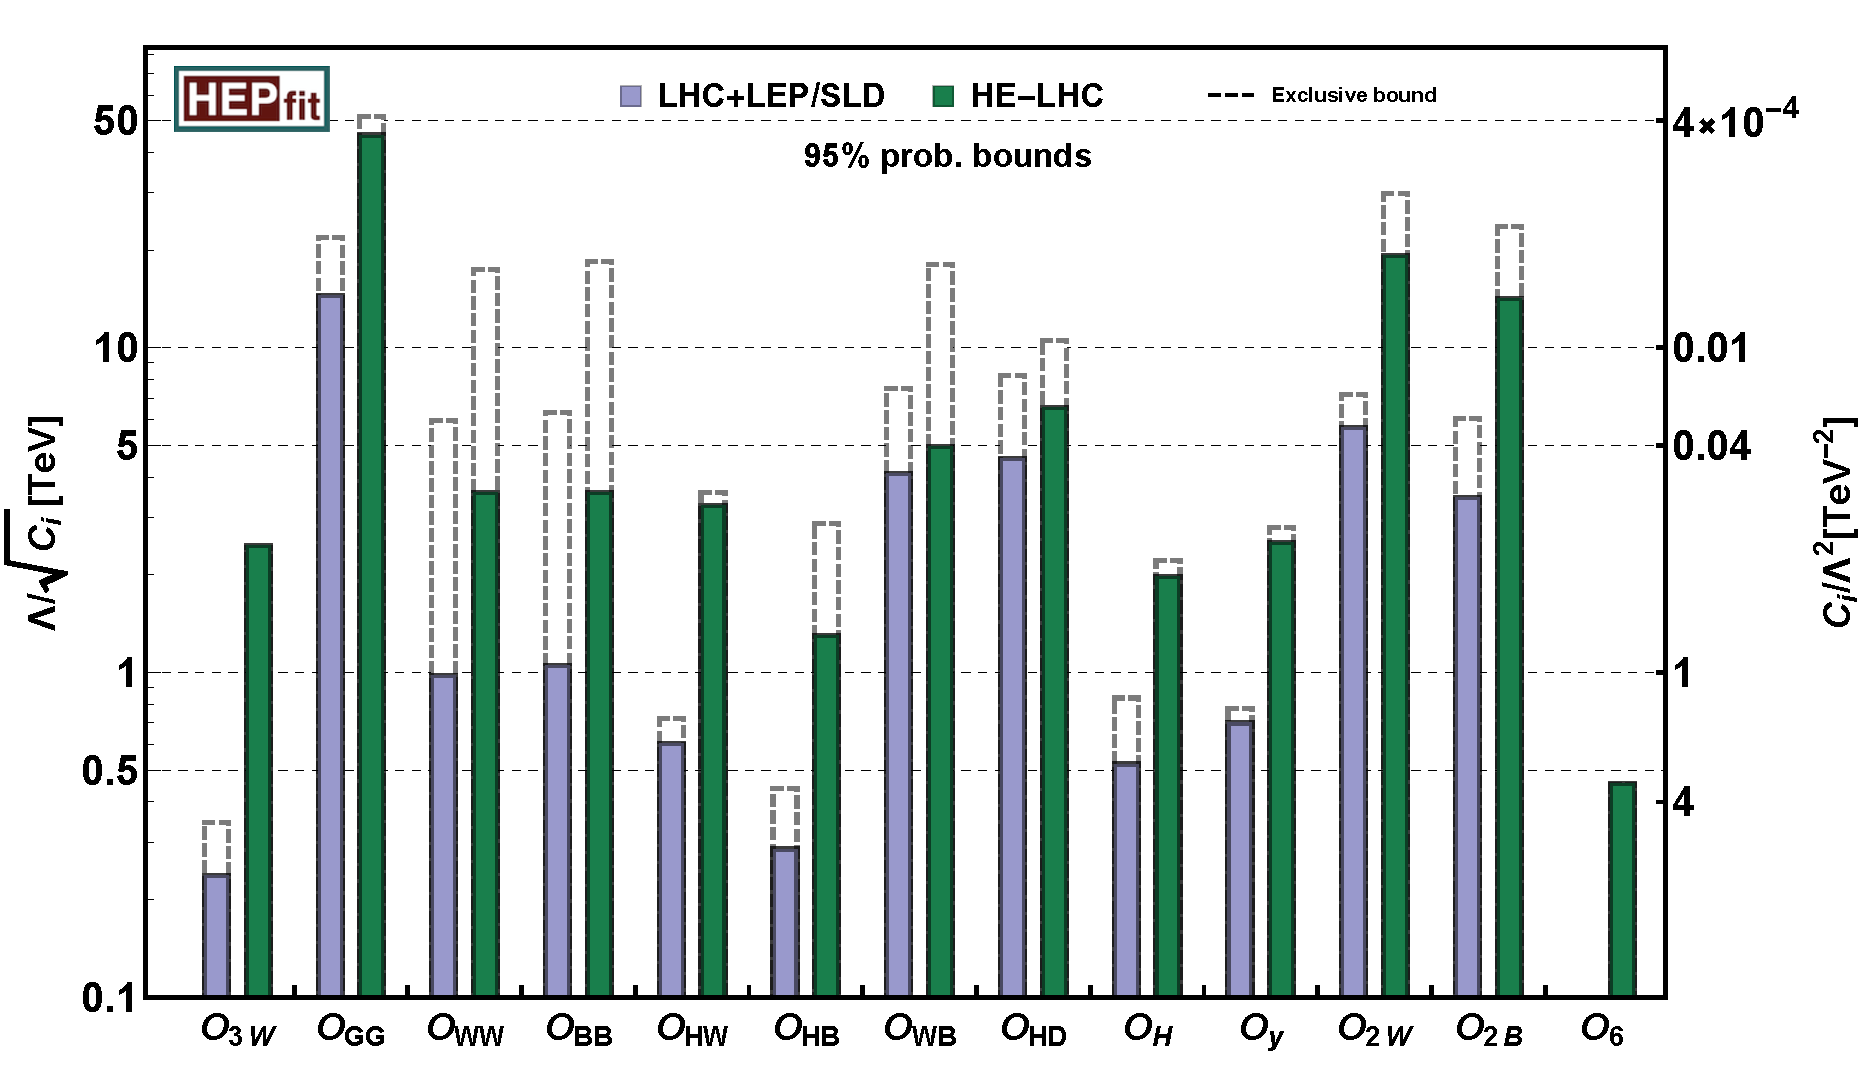
\includegraphics[width=0.85\textwidth]{section10/img/EFT_HE-LHC.pdf}
%\caption{Summary of constraints on the EFT operators considered. The shaded %bounds arise from a global fit of all operators, those assuming the existence of a single operator are labeled as "exclusive". See Section~\ref{sec8:globalfit} for details.}
%\label{fig:EFT}
%\end{figure}
Complementarily, the HE-LHC will offer unprecedented opportunities to directly test light \UTeV-scale new degrees of freedom associated to the Higgs boson and generically arising in models for electroweak symmetry breaking. 
Particularly, due to the large increase in the Higgs data set (see table \ref{tab:Hrates}), very rare exotic Higgs decays could be discovered.
%BSM theories generally predict the Higgs couplings to deviate from the SM predictions. In parallel, the HE-LHC will have a broad reach for models predicting exotic decays of the 125 \UGeV Higgs boson (e.g. decays including intermediate BSM particles that are long lived, decays including light scalars, light dark photons or axion-like particles). 
%The large variety of BSM Higgs signals studied at HL-LHC can be probed and discovered at the HE-LHC. Due to the very large production rate of the 125~\UGeV Higgs boson, the HE-LHC can have an unprecedented reach for Higgs exotic rare decays. 
For example, multi-lepton signatures could be produced from Higgs decays to light BSM particles ($X$) as dark photons, or axion-like particles: $h \rightarrow XX \rightarrow b\overline{b}\mu\mu,~4\ell$. The projected HE-LHC reach on the branching ratios of these two decay modes is estimated to be $\sim10^{-5}$ and $\sim10^{-8}$, respectively, extending the HL-LHC reach by a factor of $\sim5$ and $\sim10$, respectively (see Secs. \ref{Sec:2b2muExo}, \ref{Sec:4lExo}). As shown by these numbers, the reach of particularly clean decay modes will see a major gain at the HE-LHC mainly due to the increase in Higgs statistics (from gluon fusion production). % and $h \rightarrow  Z_D Z_D \rightarrow 4\ell$ decays (where $Z_D$ is an axion-like particle or dark photon), for which branching ratios as small as ~$10^{-5}$ and $10^{-8}$ could be probed, respectively.
At the same time, the sample of Higgs bosons produced from sub-leading production
modes in association with other SM particles (e.g. $t\bar th$) will be sizeable, increasing the discovery prospects for rare and more background limited Higgs decay signatures. Therefore, the HL/HE-LHC
Higgs exotic decay program can be uniquely sensitive to the existence of a broad range of new light
weakly coupled particles.

The increase in energy will also open up many opportunities for the direct search of new \UTeV-scale degrees of freedom associated to electroweak symmetry breaking, as new heavy Higgs bosons. In this report, we have studied, for example, the reach for $pp \rightarrow S \rightarrow hh$, with $h$ the 125~\UGeV Higgs boson and $S$ a new Higgs boson, and we have shown that the HE-LHC can extend the reach to $S$ masses that are 1.5-2 times heavier than the masses probed by the HL-LHC (see Sec. \ref{Sec.9.4.2}). Many more studies will be needed to assess the full discovery potential of the HE-LHC to extended Higgs sectors, as arising in many well motivated BSM theories.







\end{document}
